\documentclass[13pt]{beamer}
\usetheme{CambridgeUS}
\usecolortheme{dolphin}

\usepackage{microtype}
\usepackage{amsmath}
\usepackage{lmodern}
\usepackage{tikz}
\usepackage[czech,slovak]{babel}
\usepackage[utf8x]{inputenc}
\usepackage{times}
\usepackage{pgfpages}
\usepackage{amssymb}
\usepackage{graphicx}
\usepackage{listings}


\setbeameroption{show notes on second screen=right} % Both
\setbeamertemplate{show notes}{\pagecolor{yellow!5}\insertnote}\usepackage{palatino}

\usetikzlibrary{calc,trees,positioning,arrows,chains,shapes.geometric,%
    decorations.pathreplacing,decorations.pathmorphing,shapes,%
    matrix,shapes.symbols}

\title{Interpret jazyka IFJ16 (a/4/I)}
\subtitle{Semestrální projekt IFJ}
\institute{FIT VUT Brno}
\author[ Tamaškovič,Vaško,Vaško,Záleský,Zárybnický]
{Marek~Tamaškovič,Martin~Vaško, Michal~Vaško, Jiří~Záleský, Jakub~Zárybnický}
\date{14. prosince 2016}

\newsavebox{\grammarbox}

\begin{document}

\begin{frame}
  \titlepage
  \note[item]{Varianta a/4/I - Knuth–Morris–Pratt algoritmus pre vyhledáni podřetezce v řetezci, jako seřaďovací algoritmus byl použit List-Merge a tabulka symbolu byla implementovaná pomoci BVS.}
\end{frame}

\section{Úvod}

\subsection{Zadání}

\section{Architektura}

\begin{frame}{Přehled architektury}
  \begin{center}
    \begin{tikzpicture}
      [node distance = 1cm, auto,,
      every node/.style={node distance=2cm},
      force/.style={rectangle, rounded corners, draw=black, very thick,
      text width=8em, text badly centered, minimum height=3em}]

      % Draw forces
      \node [force] (center) {Hlavní řadič};
      \node [force, left=.5cm of center] (database) {Databáze};
      \node [force, below=.5cm of center] (gui) {Grafické rozhraní};
      \node [force, below=.5cm of gui] (user) {Uživatel};
      \node [force, right=.5cm of center] (server) {Server};

      \path[->,thick,shorten >=1pt,shorten <=1pt]
      (center) edge (database)
      (center) edge (gui)
      (center) edge (server)
      (gui) edge (center)
      (server) edge (center)
      (database) edge (center)
      (user) edge (gui)
      (gui) edge (user);

    \end{tikzpicture}
  \end{center}
\end{frame}

\begin{frame}{Datové typy (AST)}
\end{frame}

\begin{frame}{Hierarchie typů}
\end{frame}

\section{Komponenty}
\subsection{Lexer}

\begin{frame}{Poznámky k implementaci (změnit název?)}
\begin{itemize}
 \item vytvoření makra getchar
 \item token dokáže posílat informace o řádku a sloupci na kterém se daný znak nachází
 \item implementovane rozšíření jako UNARY, BOLOP, CYCLES
 \item mírně problémy s rozšířením BASE, kde bylo třeba dodatečně implementovat funkci hexToDbl
  \note[item]{Lexikálna analýza funguje na princípe konečného automatu. Ten načíta zo vstupného súboru znaky, lexikálna analýza ich vyhodnotí a posiela ako tokeny do syntaktického analyzátora. Tokeny obsahujú informácie o type a obsahu. Taktiež sme si ale implementovali aj macro GetChar vďaka ktorému dokáže náš token posielať nielen základne informácie o type ci obsahu ale pridáva k nim aj ďalšie informácie o riadku a stĺpci na ktorej sa tieto znaky v interpretovanom súbore nachádzajú a výrazne tak uľahčuje prácu syntaktickému analyzátoru.}
  \note[item] {Ako si môžete všimnúť aj v diagrame ,implementovali sme aj všetky dostupne rozšírenia. Menovite BOOLOP , Unarne ale aj cykly typu for a do-while. Menší problém však bol s rozšírením BASE. Konkrétne s prevodom hexadecimálnej sústavy v desatinnom tvare. Tu sme museli implementovať funkciu hexToDbl ktorá to následne prekonvertovala do desiatkovej sústavy.}
\end{itemize}
\end{frame}

\begin{frame}{Stavový diagram lexeru}
  \begin{center}
    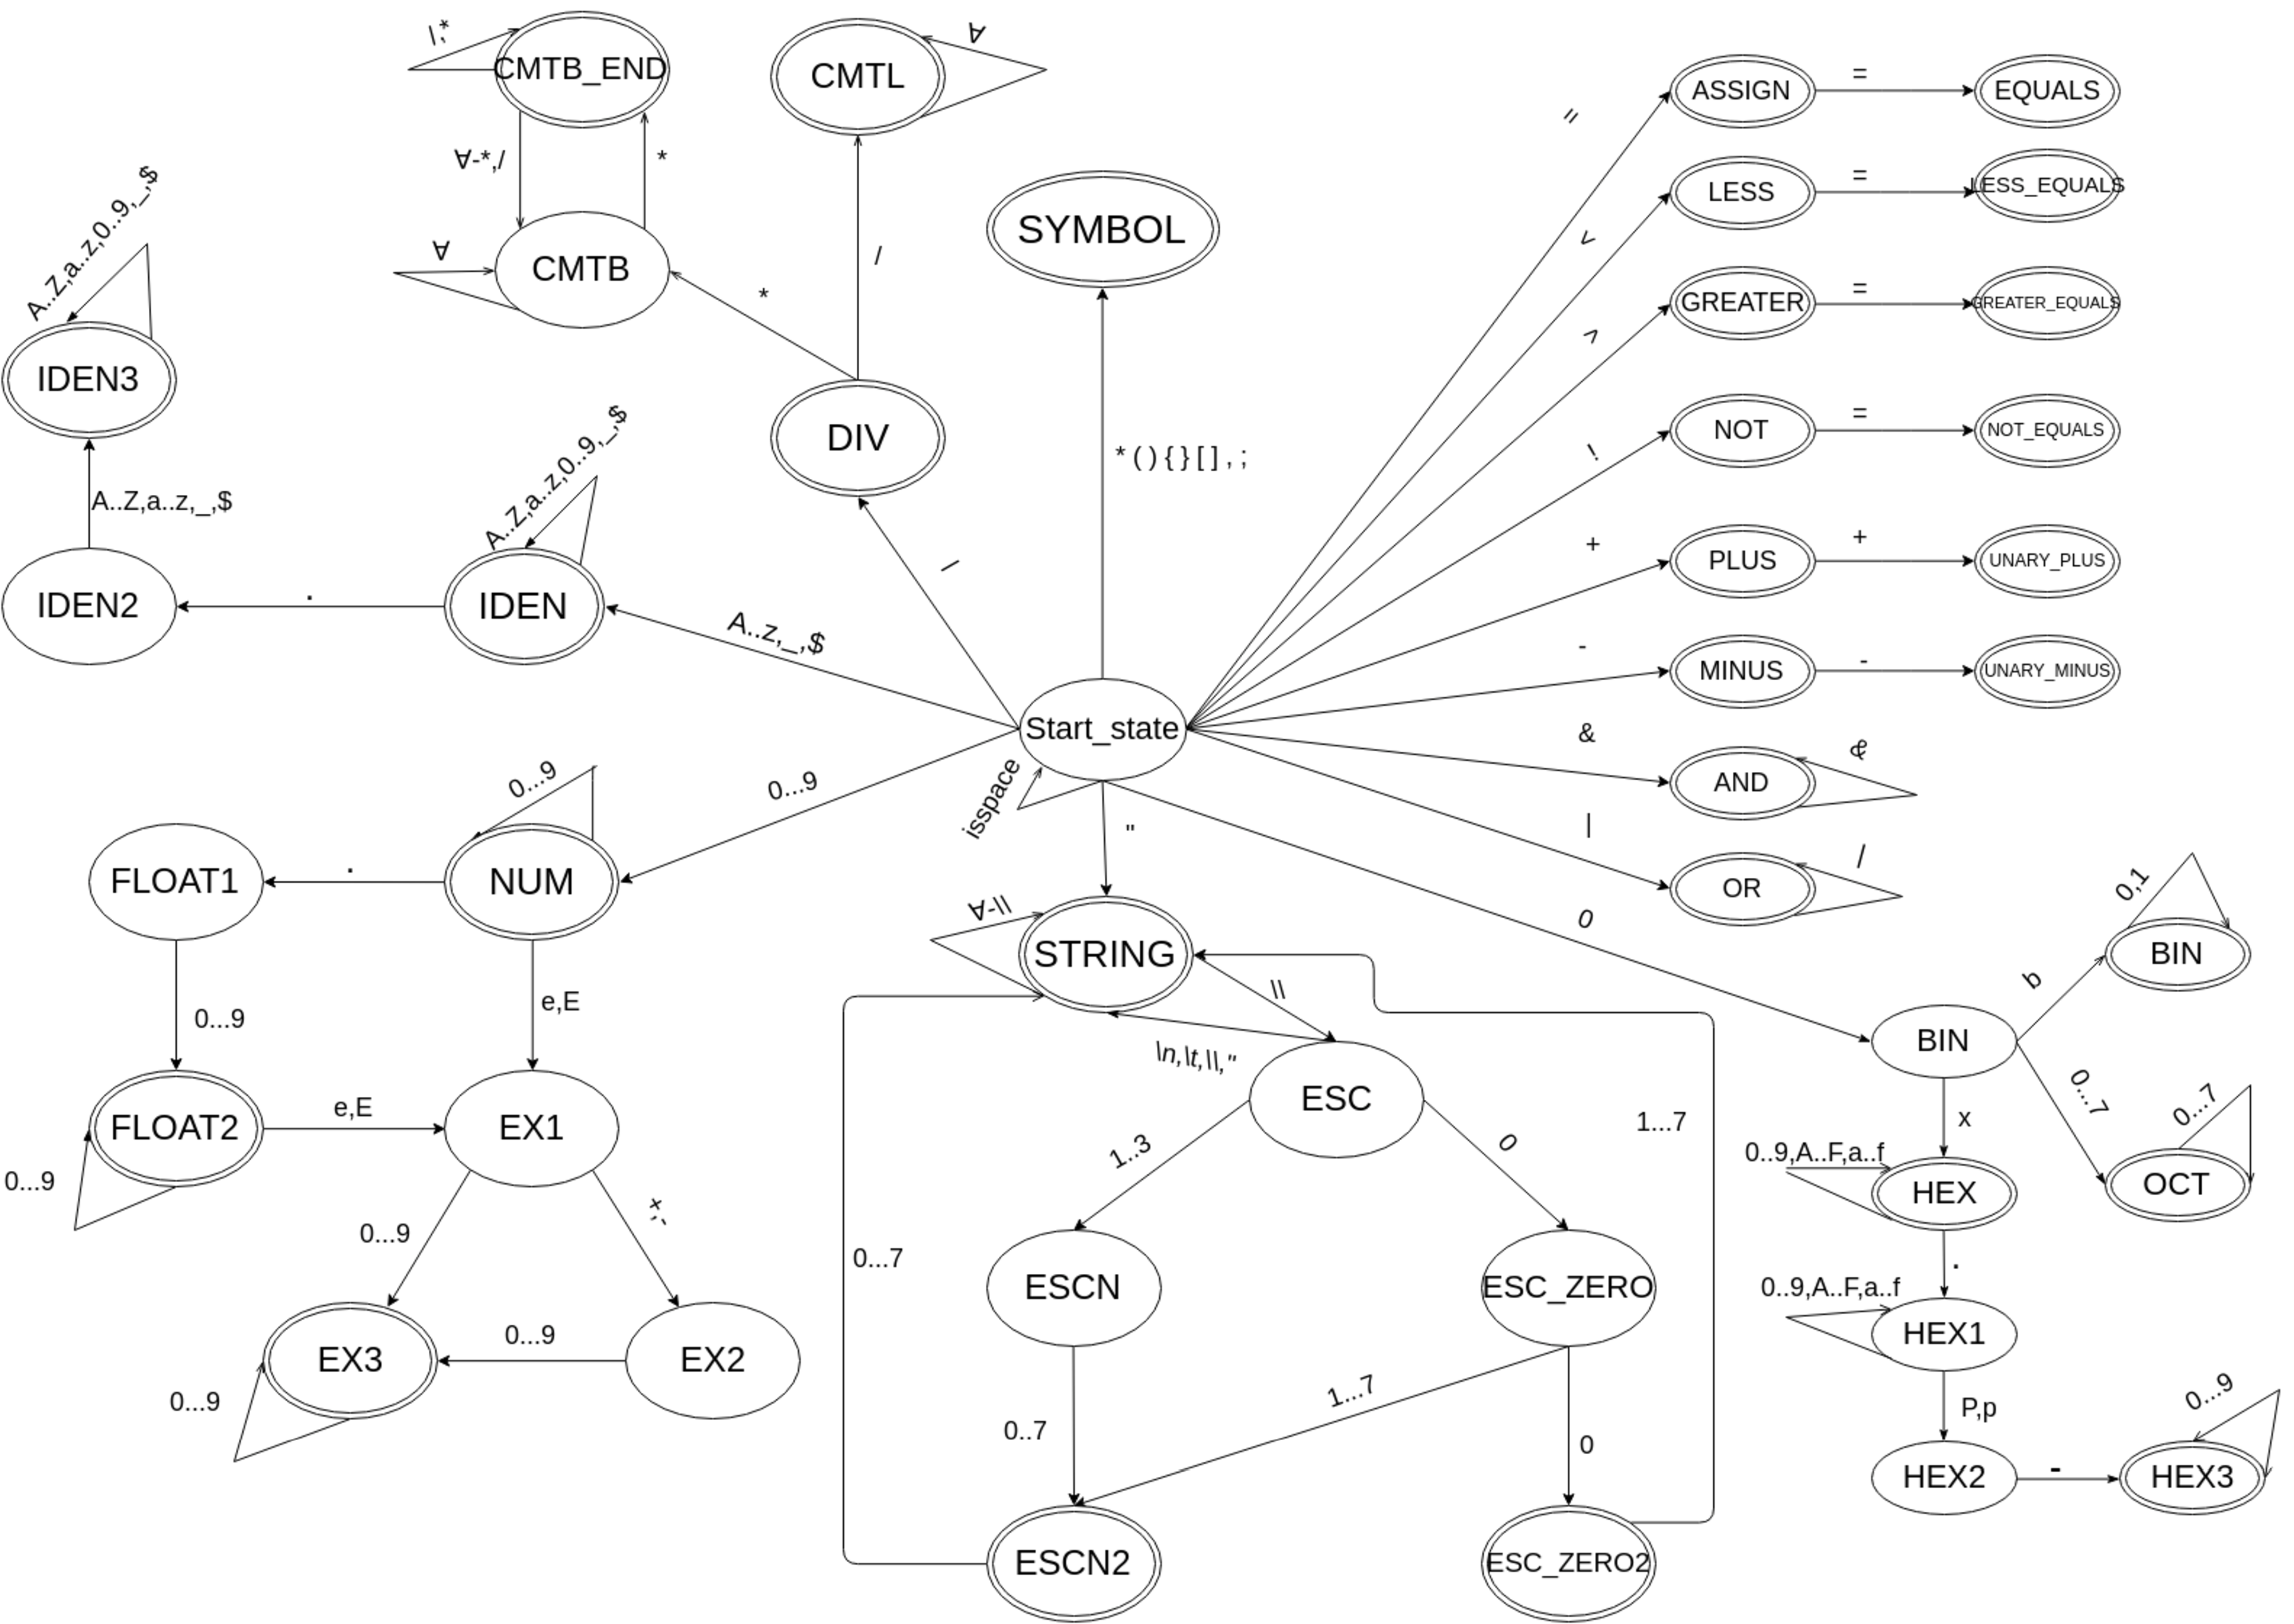
\includegraphics[width=0.8\textwidth]{img/lex1.pdf}
  \end{center}
\note[item]{ Čo sa týka diagram ktorý vidíte na obrazovke, urobil som par zmien aby sa zvýšila prehľadnosť diagramu. Konkrétne pri Symboloch kde som vytvoril jeden stav a pomenoval ho symbol a tam poslal všetky symboly ktoré nepotrebovali implementovať stav v automate a taktiež pri ďalších symboloch ako >,<,+++,-- atď.(o ktoré symboly sa jedna je  vidno na diagrame, pravá strana) kde som miesto jedného stavu pridal aj druhy ktorý v kóde nie je a to preto aby som názorne ukázal ako prebieha jednotlivé načítanie znakov v lexikálnej analýze i aj keď nie sú už súčasnou stavov avšak úplne zodpovedajú tomu ako lexikálna analýza funguje.}
\end{frame}

\subsection{Syntaktická analýza}

\begin{frame}{Podrobnosti o implementaci Syntaktické analýzy}
  \begin{itemize}
  \item analýza rekurzivním sestupem, precedenční analýza
  \item stávající implementace je druhá, původní byla rekurzivním sestupem všude
  \item nová implementace mnohem delší a méně elegantní, i když asi rychlejší
  \item bez použití maker by bylo kódu cca o 300\% víc
  \item např. \texttt{expectSymbol(l, SYM\_SEMI);} odpovídá 15 řádkům kódu
  \item umožňuje skoro přímý přepis gramatiky do C
  \item UNARY - podmíněný přepis \textbf{-} na \textbf{u-} (za znaky \$, ( a za operátory)
  \end{itemize}
\end{frame}

\begin{frame}[fragile]{LL gramatika}
\begin{lrbox}{\grammarbox}%
    \begin{lstlisting}%
ifj16 = \$ | class ifj16
class = "class" "{" classBody
classBody = "}" | "static" type simpleId classBody'
classBody' = ";"
           | "=" expression ";"
           | "(" declarationList "{" functionBody
functionBody = "}"
              | type simpleId(q) functionBody'
              | command
functionBody' = ";" | "=" expression ";"
command = "if" "(" expression ")" command
        | "while" "(" expression ")" command
        | "do" command "while" "(" expression ")" ";"
        | "for" "(" type simpleId for'
        | "return" return'
        | "{" commandList
        | "break" ";"
        | "continue" ";"
        | anyId command'
for' = ";" for'' | "=" expression ";" for''
for'' = expression ";" anyId "=" expression ")" command
return' = ";" | expression ";"
commandList = "}" | command commandList
command' = "(" argumentList ";" | "=" expression ";"
declarationList  = ")" | type simpleId declarationList'
declarationList' = ")" | "," type simpleId declarationList'
argumentList  = ")" | expression argumentList'
argumentList' = ")" | "," expression argumentList'
type = "int" | "double" | "boolean" | "String" | "void"
anyId = simpleId | compoundId
    \end{lstlisting}%
\end{lrbox}%
\scalebox{0.52}{\usebox{\grammarbox}}
\end{frame}

\begin{frame}{Precedenční tabulka}
\scalebox{0.55}{
\begin{tabular}[pos]{r|l|l|l|l|l|l|l|l|l|l|l|l|l|l|l|l|l|l|l|l|l|l|l}
    &(&)&++&--&u-& !& *& /& +& -& <& >&<=&>=&==&!=&\&\&&$\|$&id&li&tf&,& \$ \\
    (& L& E& L& L& L& L& L& L& L& L& L& L& L& L& L& L& L& L& L& L& L& E& O \\
    )& O& G& O& O& O& O& G& G& G& G& G& G& G& G& G& G& G& G& O& O& O& G& G \\
    ++& O& G& G& G& O& O& G& G& G& G& G& G& G& G& G& G& G& G& L& O& O& G& G \\
    --& O& G& G& G& O& O& G& G& G& G& G& G& G& G& G& G& G& G& L& O& O& G& G \\
    u-& L& G& O& O& G& G& G& G& G& G& G& G& G& G& G& G& G& G& L& G& L& O& G \\
    !& L& G& O& O& G& G& G& G& G& G& G& G& G& G& G& G& G& G& L& G& L& O& G \\
    *& L& G& L& L& L& L& G& G& G& G& G& G& G& G& G& G& G& G& L& L& L& G& G \\
    /& L& G& L& L& L& L& G& G& G& G& G& G& G& G& G& G& G& G& L& L& L& G& G \\
    +& L& G& L& L& L& L& L& L& G& G& G& G& G& G& G& G& G& G& L& L& L& G& G \\
    -& L& G& L& L& L& L& L& L& G& G& G& G& G& G& G& G& G& G& L& L& L& G& G \\
    <& L& G& L& L& L& L& L& L& L& L& G& G& G& G& G& G& G& G& L& L& L& G& G \\
    >& L& G& L& L& L& L& L& L& L& L& G& G& G& G& G& G& G& G& L& L& L& G& G \\
    <=& L& G& L& L& L& L& L& L& L& L& G& G& G& G& G& G& G& G& L& L& L& G& G \\
    >=& L& G& L& L& L& L& L& L& L& L& G& G& G& G& G& G& G& G& L& L& L& G& G \\
    ==& L& G& L& L& L& L& L& L& L& L& L& L& L& L& G& G& G& G& L& L& L& G& G \\
    !=& L& G& L& L& L& L& L& L& L& L& L& L& L& L& G& G& G& G& L& L& L& G& G \\
    \&\&& L& G& L& L& L& L& L& L& L& L& L& L& L& L& L& L& G& G& L& L& L& G& G \\
    $\|$& L& G& L& L& L& L& L& L& L& L& L& L& L& L& L& L& L& G& L& L& L& G& G \\
    id& E& G& G& G& O& O& G& G& G& G& G& G& G& G& G& G& G& G& O& O& O& G& G \\
    literal& O& G& O& O& O& O& G& G& G& G& G& G& G& G& G& G& G& G& O& O& O& G& G \\
    true/false& O& G& O& O& O& O& G& G& G& G& G& G& G& G& G& G& G& G& O& O& O& G& G \\
    ,& L& E& L& L& L& L& L& L& L& L& L& L& L& L& L& L& L& L& L& L& L& E& O \\
    \$& L& O& L& L& L& L& L& L& L& L& L& L& L& L& L& L& L& L& L& L& L& O& O
\end{tabular}
}
\end{frame}

\subsection{Podrobnosti o implementaci Sémantické analýzy}

\begin{frame}{Sémantická analýza}
  \begin{itemize}
    \item V projekte používame funkcionálné programovanie.
    \item Nachádzajú sa tam rôzne kontroly napr.: \texttt{getExpressionType, isAssignCompatible}
  \end{itemize}
\end{frame}

\subsection{Interpret}

\begin{frame}{Podrobnosti o implementaci Interpretu}

    % FIXME cestina

  \begin{itemize}
    \item Makra opět tvoří velkou část kódu
    \item \texttt{\#define I(x) (x)->data.integer}
    \item \texttt{I(result) = I(left) + I(right)}
    \item Cykli jsou implementované stejným spůsobem ako v jazyce C
    \item \texttt{CYCLE\_INNER(...)} (break, continue, return handling)
    \item \texttt{while (evalExpression(...)) \{ CYCLE\_INNER(...); \}}
  \end{itemize}
  \note[item] {Dovolili jsme si použít GOTO jako nástroj pro vypsáni erroru i když Djisktra ho považuje za škodlivej. Ulehčili jsme si přitom práci s cykly, které se znova pomoci makra usnadnilo}
  \note[item]{Doslovný přepis cyklů - for v ifj16 je for v C apod.}
\end{frame}

\begin{frame}{Zajimavosti o implementaci Interpretu}
  \begin{itemize}
    % FIXME cestina
    \item Interpret interpretuje přímo AST a ne tříadresný kód
    \item We didn't consider GOTO harmful (Dijkstra, 1968)
    \item Základní garbage collector (GC pouze při skončení)
    \item Padl nejeden návrh na implementaci skryté funkcionality \texttt{ifj16.launchMissiles()}
  \end{itemize}
  \note[item] {AST - interpretace nemusí být volána ze syn. an.}
  \note[item] {Goto - Museli jsme použít goto pri cyklech. Nebylo jíne východisko :) }
  \note[item] {GC - všechny malloc, calloc, realloc, free jsou nahrazeny ekvivalentmi v GC}
  \note[item] {Návrh byl potlačen násilím}
\end{frame}

\section{Algoritmy}

\begin{frame}{Podrobnosti o implementaci Algoritmů}

  \begin{itemize}
    \item Seřazení prvků v poli - List-Merge sort $\mathcal{O}(n log(n))$
    \item Najít podřetězec v řetězci - Knutt-Morris-Pratt $\mathcal{O}(n)$
    \item Tabulka symbolů - BVS - vyhledání $\mathcal{O}(log (n))$
  \end{itemize}
   \note[item] {List-Merge Princip založen jak už název napovídá na mergování (slévání). Před samotným mergováním, je vytvořeno pomocné pole do něhož indexy nebo nuly umístěny jsou. Nula nechť znakem je pro konec posloupnosti neklesající. Po najití všech neklesajících posloupnosí jsou jejich začátky vloženy do datové struktury typu seznam a zařazeny za sebou tvoří frontu. Při mergování vezmeme dva první prvky a postupně je spojíme do jednoho seřazeného seznamu, který následně na konec vložíme. Takto postupujeme dokud nezůstane už jen jeden seznam, který obsahuje vše a seřazené. Pozn. k Implem. Při vybírání prvních dvou kontrolujeme zda nejde o seznam vložený při přípravě jako konečný, aby nedošlo ke spojení seznamů přes hranu pole. Původně to tak bylo řešeno, ale kvůli neočekávanému chování to zavrženo bylo. Dále také pro jednoduchost zpracování je zajištěno (v případě nepravdivosti se před merg. prohodí), že seznam, který je více vlevo (má nižší index), je považovám při mergování za první a tudíž po slití umístěn na konec fronty.}
  \note[item] {KMP nejprve vyhledává podřetězce v hledaném podřetězci a uklada pozice podřetězců do pomocného pole. Po zkompletování pomocného pole začne vyhledávání v zadaném řetězci. Dochází k porovnávání a narazí-li se na neshodu vrátí se pouze o část specifikovanou v pomocném poli a pokračuje v porovnávání. Může nastat situace kdy ani posunutí o určitý poček znaků nepomůže a tak se u hledaného podřetězce začne od začátku. Urychlení spočívá právě v tom, že se nemusí vždy začínat od začátku. Jelikož začíná naše pole od 0, je jako znak pro návrat na začátek -1. (Ve videu 0, ale maji pole od 1)}
  \note[item] {Binární vyhledávací strom - základem je vkladání a nalezení uzlu, AVL strom sme se rozhodli vyvažovat z důvodu mnoha uzlů (hlavně vestavěné funkce), a tím pádem rychleji daný uzel najít. - spíše teoretické cvičení, na skutečnou rychlost nemá velký vliv}
\end{frame}

% výcuc o List-merge sort - http://dudka.cz/studyIAL
% Dobře vysvětlený knutt-moriis-pratt - https://www.youtube.com/watch?v=HaAu5ZGj6fc

\section{Závěr}
\begin{frame}{Statistiky - Git}
  \begin{center}
    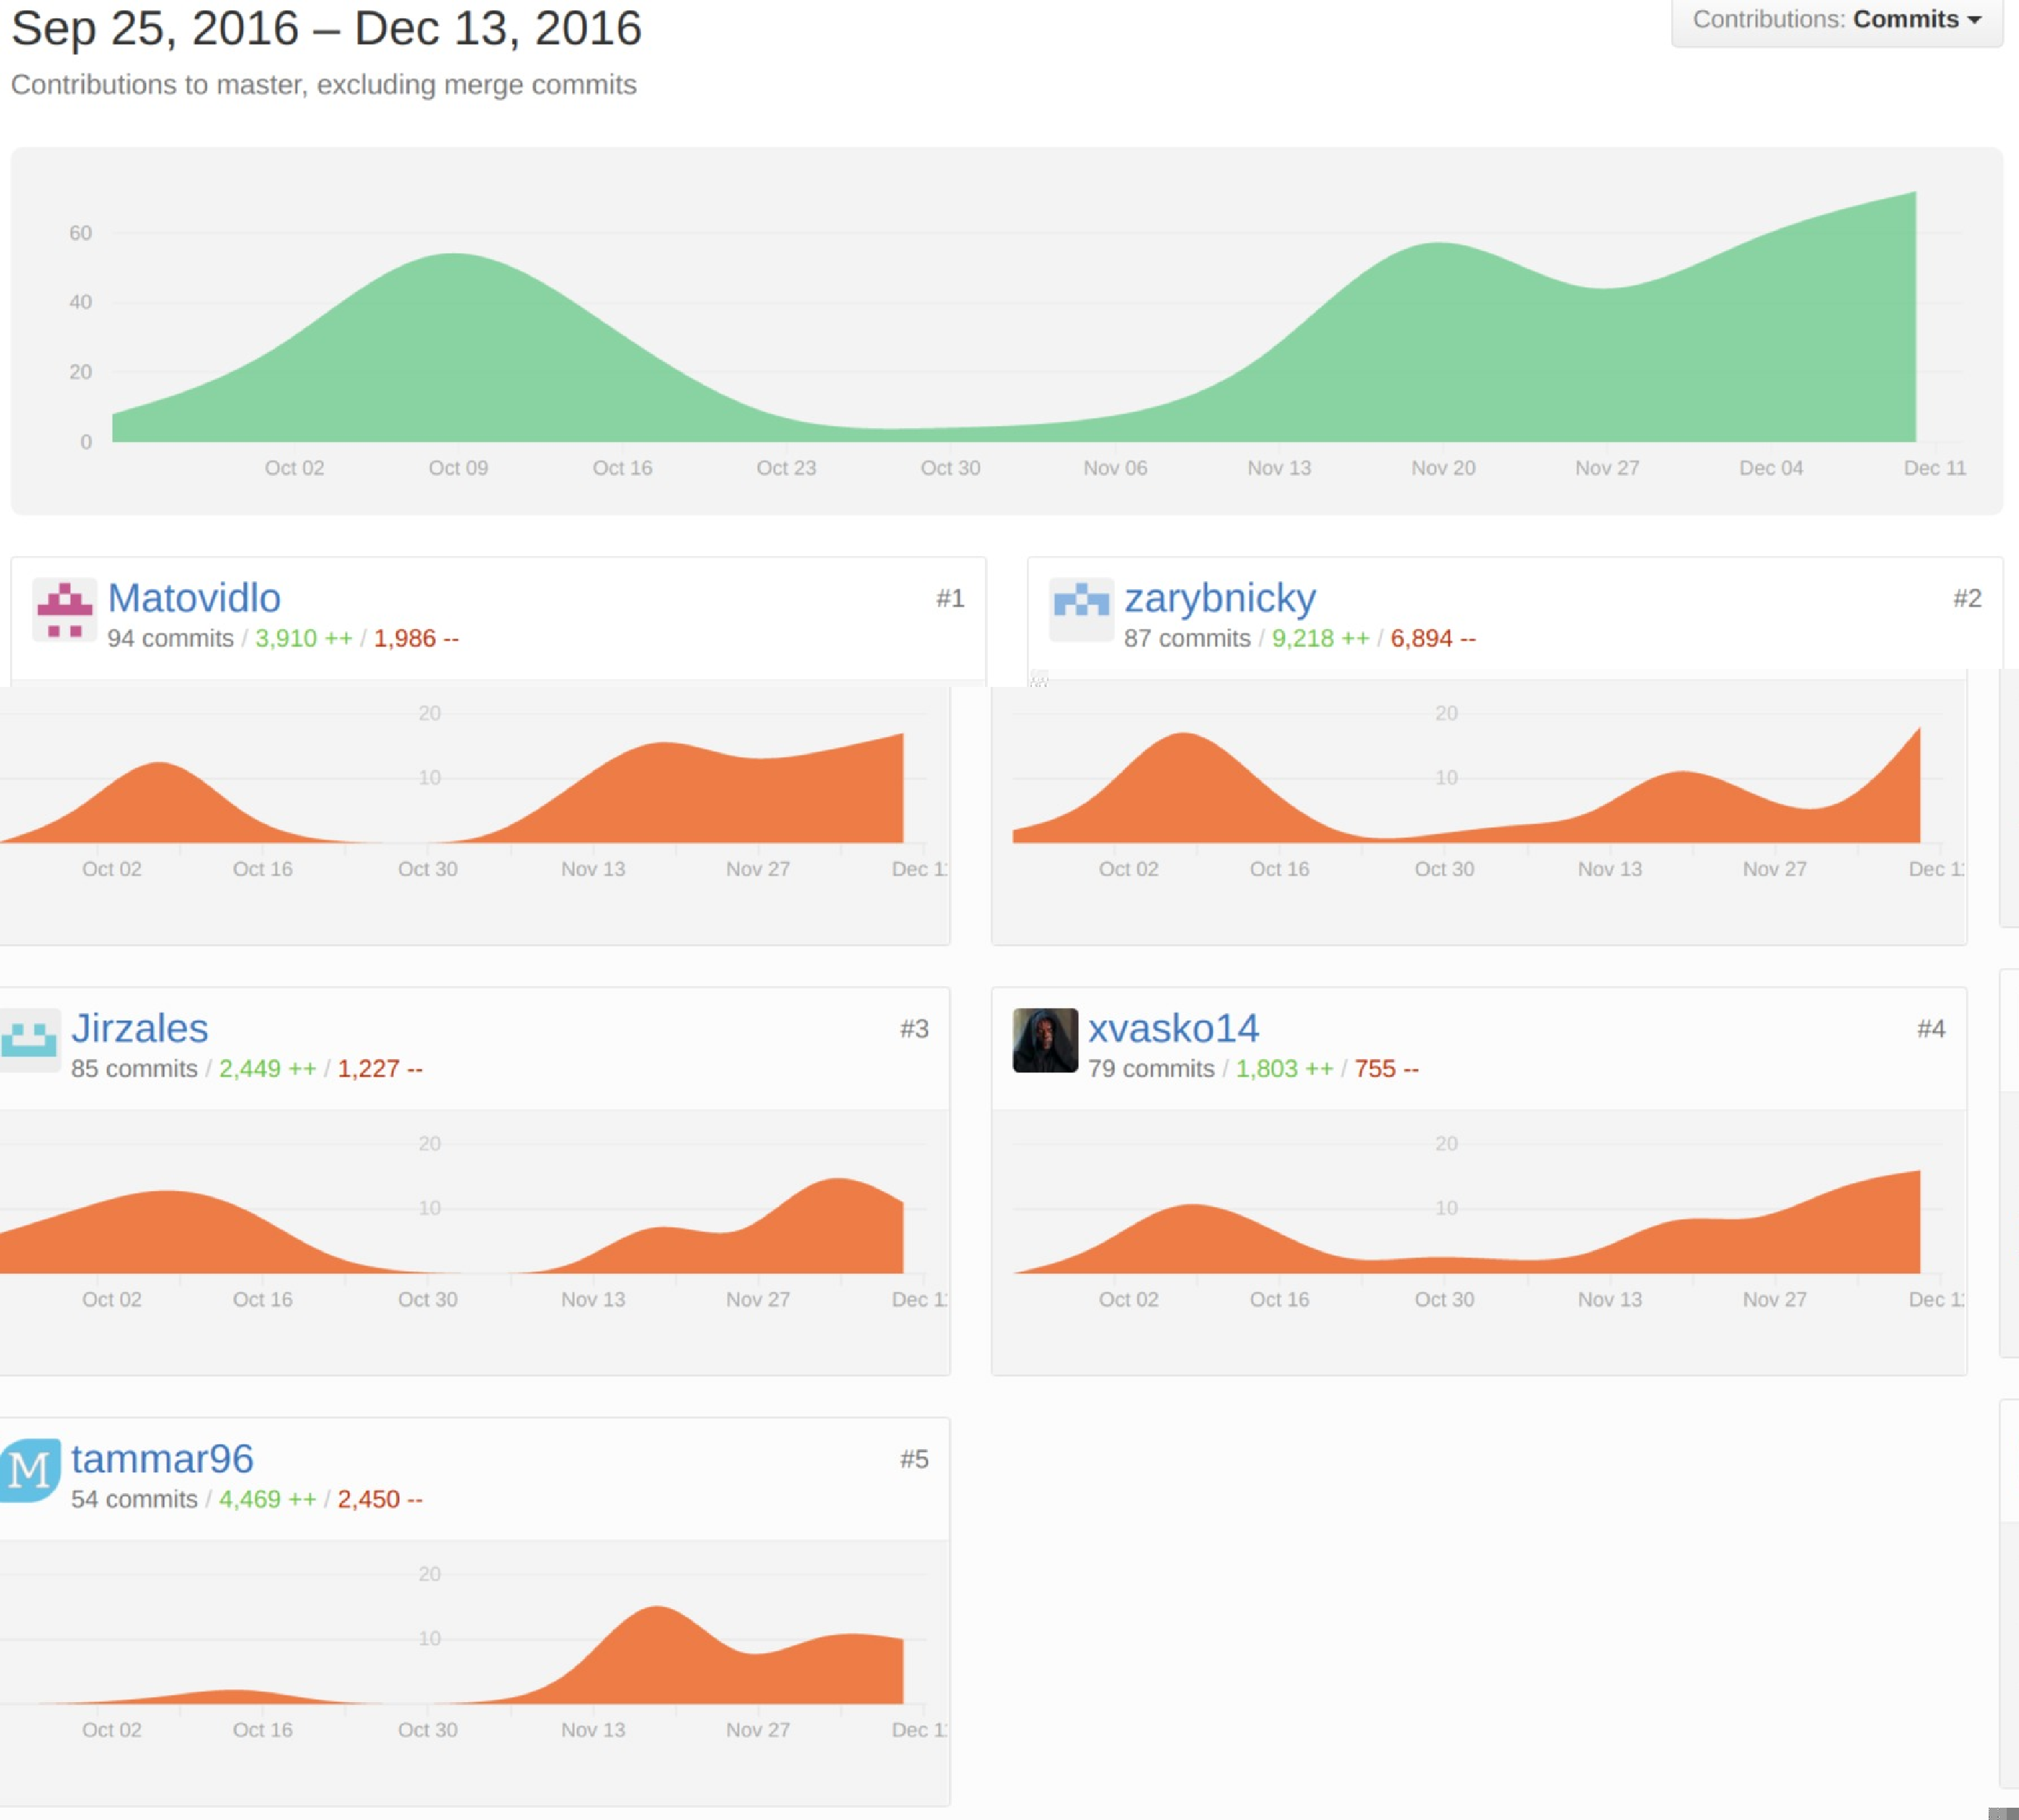
\includegraphics[width=0.65\textwidth]{./img/git_commit.pdf}
  \end{center}
\end{frame}

\begin{frame}{Statistiky - Git}
  \begin{center}
    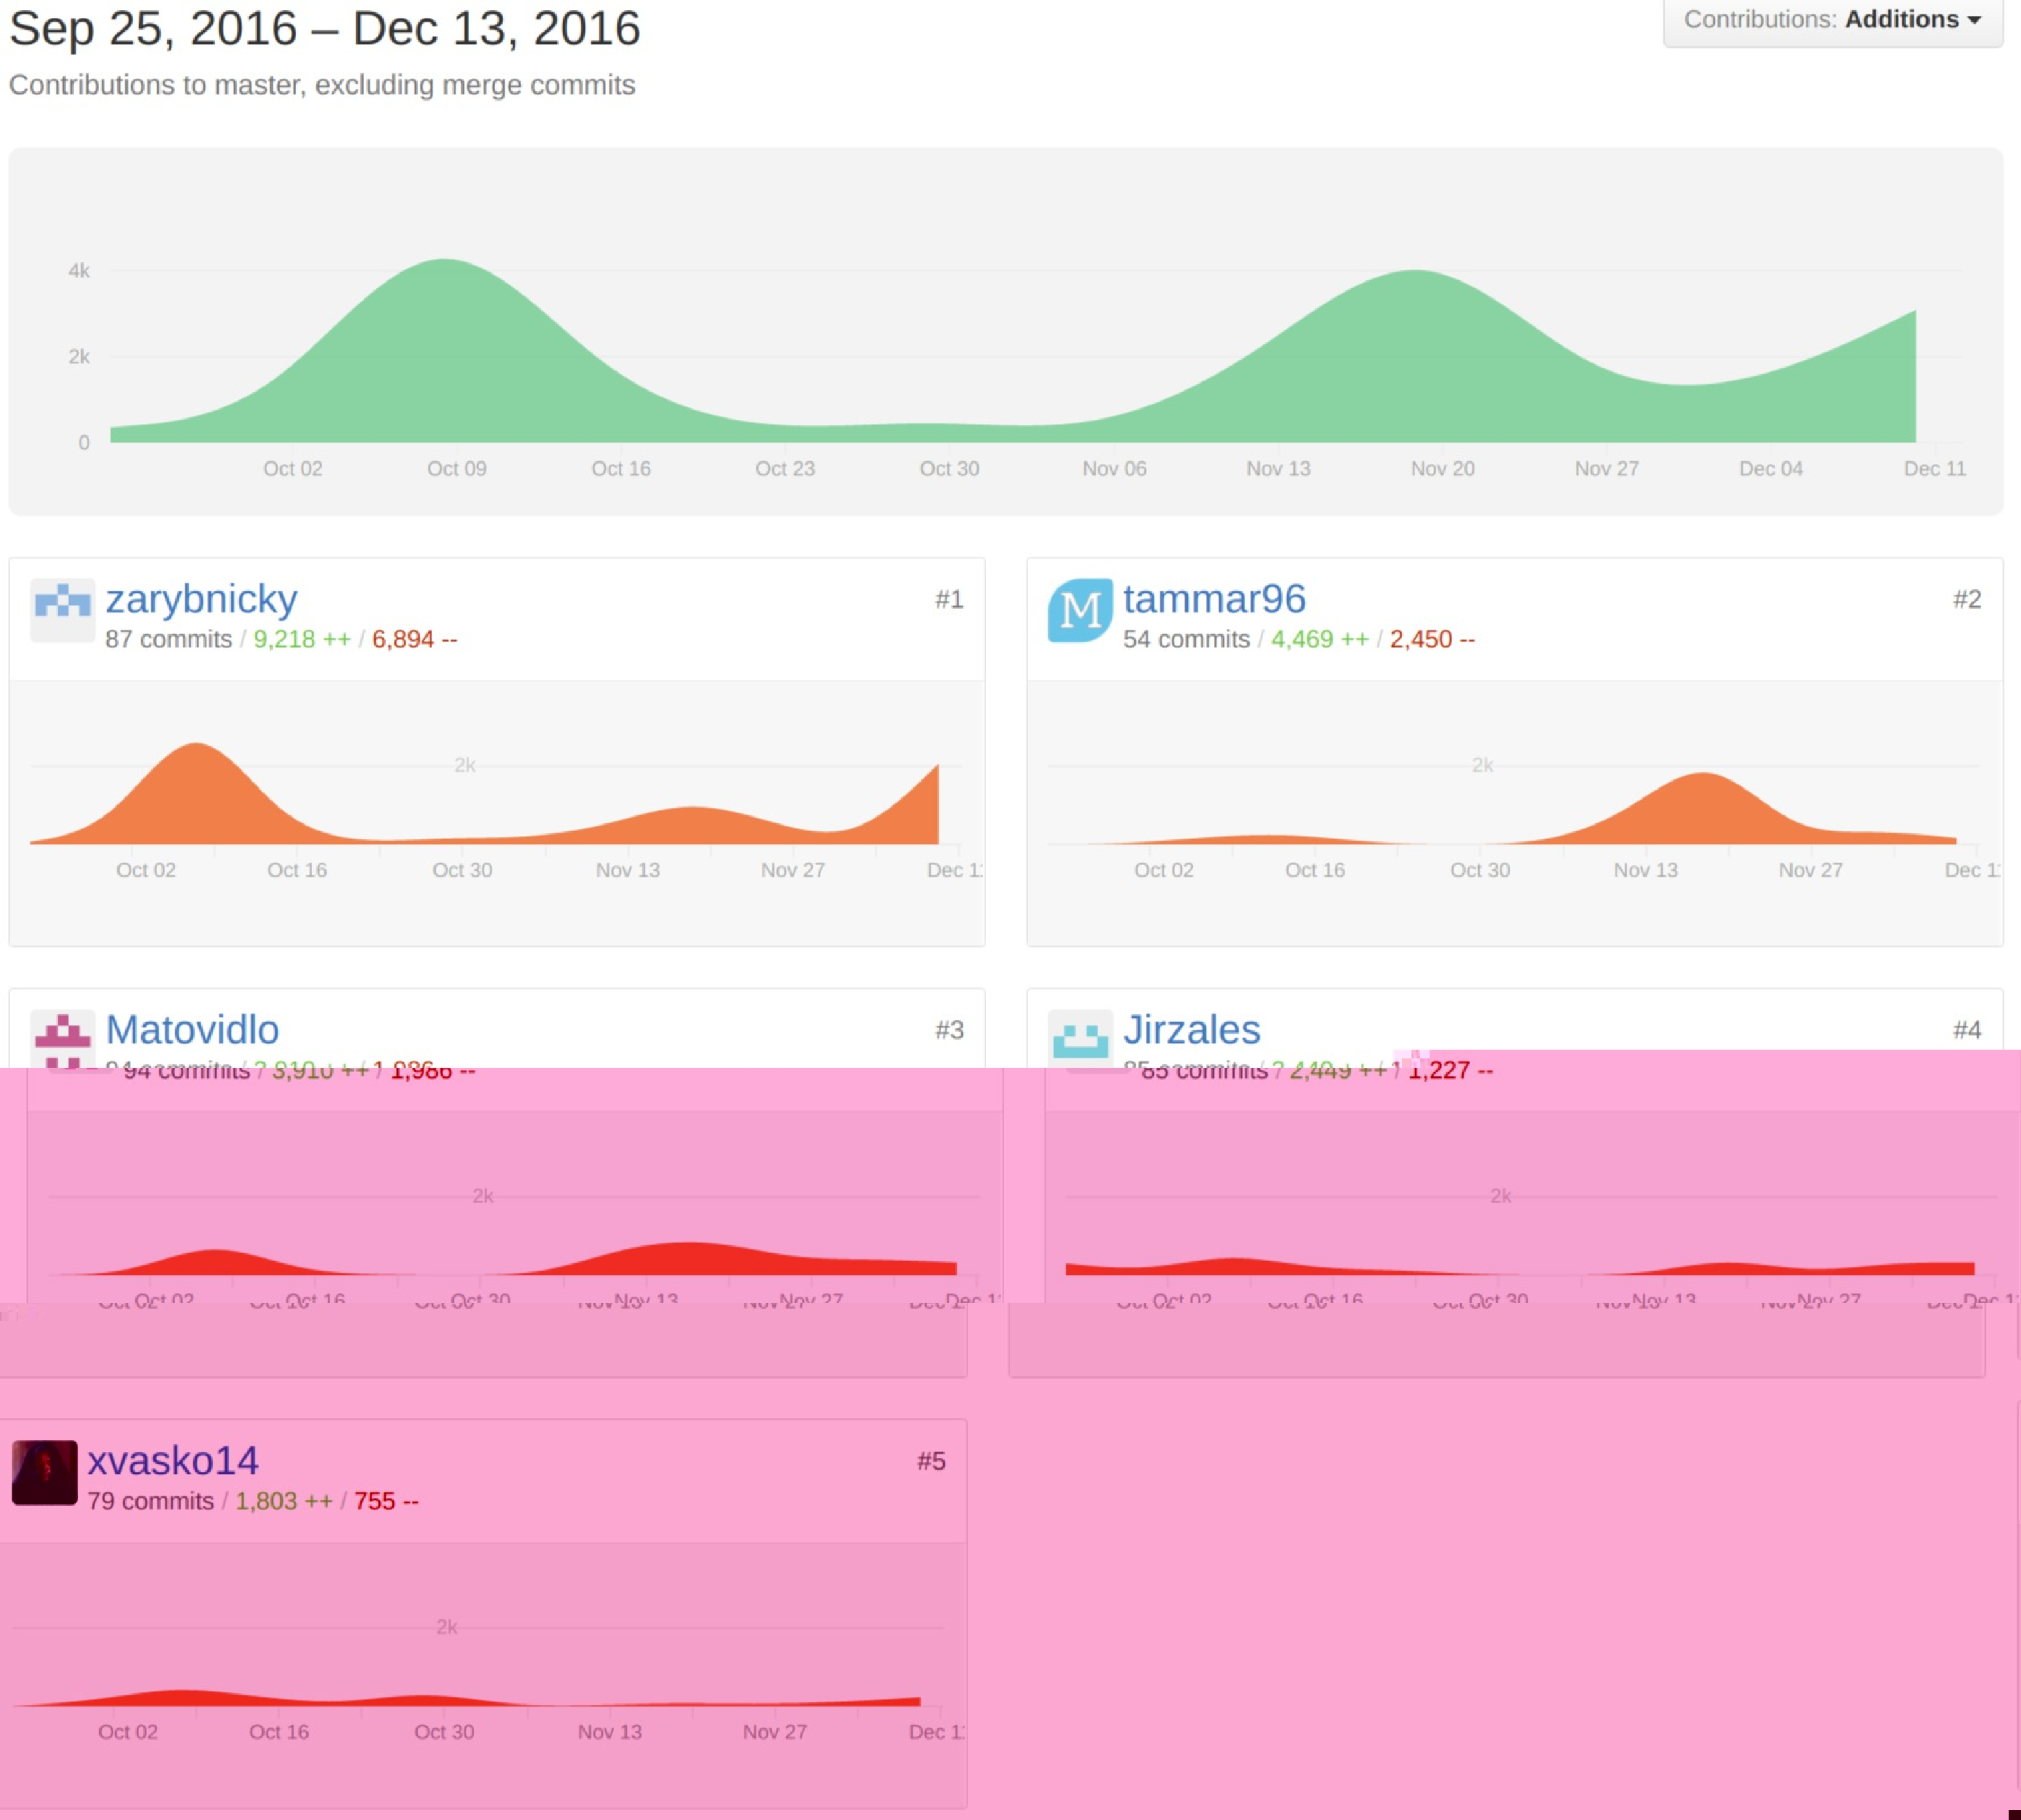
\includegraphics[width=0.65\textwidth]{./img/git_additions.pdf}
  \end{center}
\end{frame}

\begin{frame}{Statistiky - Git}
  \begin{center}
    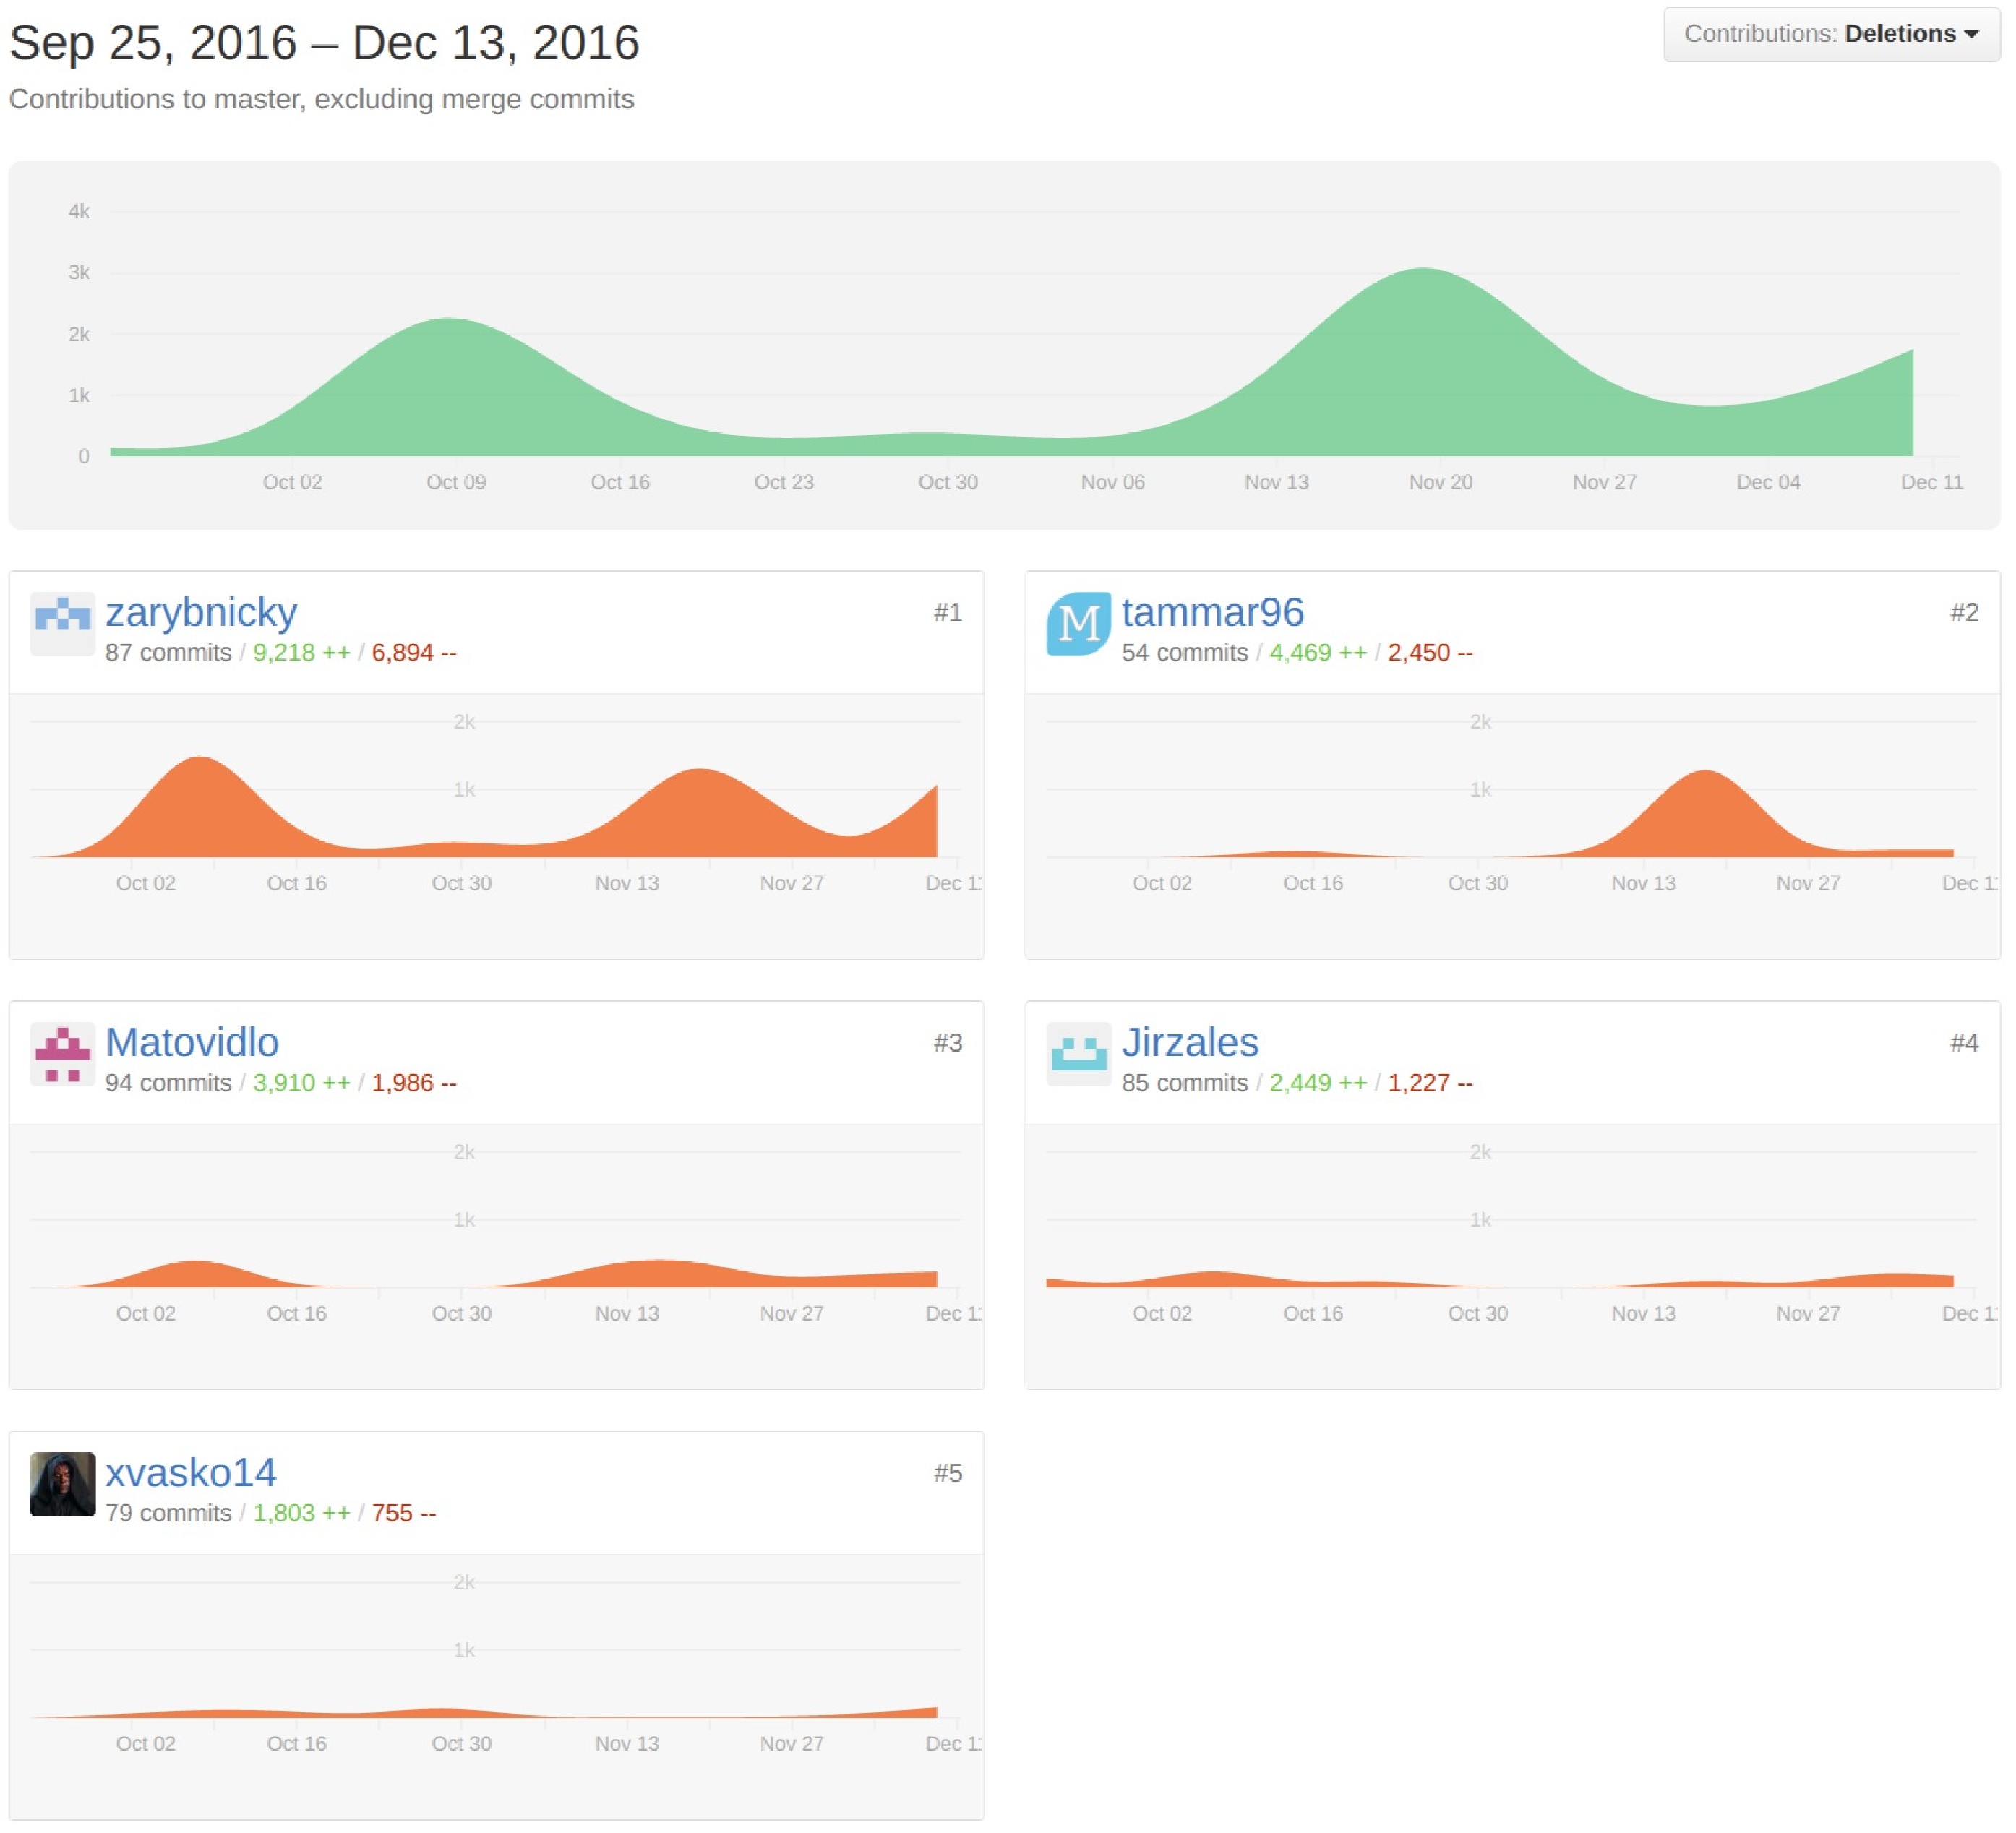
\includegraphics[width=0.65\textwidth]{./img/git_del.pdf}
  \end{center}
\end{frame}

\begin{frame}{Statistiky, očekávání, rozpočet a zhodnocení}
\begin{itemize}
\item Počet súborov: \textbf{97} (\textbf{27} v C)
\item celkový počet riadkov zdrojového kódu: \textbf{6622} (\textbf{5272} v C)
\item Počet Git commitov: \textbf{396}
\end{itemize}

\begin{itemize}
\item Plánované datum dokončení - 31.10.
\item Skutečné datum dokončení - 11.12.
\item Plánovaný peněžní zisk - 0 CZK/EUR
\item Finanční stav po ukončení projektu - záporný
\end{itemize}

\end{frame}

\end{document}
